\documentclass[11pt,a4paper]{article}
\usepackage[margin=0.8in]{geometry}
\usepackage{amsmath,booktabs,longtable,array,enumitem,xcolor,hyperref,listings,tikz}
\usetikzlibrary{arrows.meta,positioning,shapes.geometric,fit,calc,trees,matrix}
\hypersetup{colorlinks=true,linkcolor=blue,urlcolor=blue}
\setlist[itemize]{leftmargin=1.5em}
\setlist[enumerate]{leftmargin=1.7em}
\lstset{basicstyle=\ttfamily\small,breaklines=true,frame=single,columns=fullflexible}
\tikzset{
process/.style={draw,rounded corners,minimum width=3.3cm,minimum height=.8cm,align=center},
datastore/.style={draw,cylinder,shape border rotate=90,aspect=.25,minimum width=2.7cm,minimum height=1cm,align=center},
entity/.style={draw,rounded corners,minimum width=2.3cm,minimum height=.7cm,align=center},
decision/.style={draw,diamond,aspect=2,minimum width=2.6cm,minimum height=1cm,align=center},
flow/.style={-{Stealth[length=3mm]},thick},
relation/.style={-{Stealth[length=2.5mm]},thick}
}
\title{\textbf{Cross-Border Tax Intelligence with Graph-RAG}\\\large Technical Architecture, Knowledge Modeling, Retrieval Workflows, and Reference Implementation}
\author{}\date{}
\begin{document}\maketitle
\begin{abstract}
This reference architecture describes a tax intelligence system combining conventional Retrieval-Augmented Generation with graph-based retrieval. Jurisdiction-local questions can use scoped semantic retrieval. Cross-border questions require relationship-aware retrieval across tax residency, asset location, source-country taxation, residence-country taxation, treaties, withholding, foreign tax credits, refunds, reporting obligations, legal authority, and effective dates.
\end{abstract}
\tableofcontents\newpage

\section{Problem Definition}
A local query such as ``How are dividends from Indian listed companies taxed for an Indian resident?'' may primarily require retrieval from one jurisdictional corpus:
\[
\text{Query}\rightarrow\text{India Tax VectorDB}\rightarrow\text{Legal Evidence}\rightarrow\text{LLM}.
\]
A cross-border query such as ``An Indian tax resident owns US shares, receives dividends with US tax withheld, and wants to understand Indian treatment and possible relief'' requires connected knowledge across multiple legal systems.

The architectural question therefore changes from:
\begin{quote}Which documents are semantically similar to the question?\end{quote}
to:
\begin{quote}Which jurisdictions, legal concepts, treaties, tax events, and reporting obligations are structurally connected to this fact pattern and must therefore be considered together?\end{quote}

\section{Storage Architecture}
\begin{center}
\begin{tabular}{p{3.2cm}p{10cm}}\toprule
Storage & Primary responsibility\\\midrule
Vector Database & Semantic retrieval of statutes, regulations, tax authority guidance, treaty text, procedures, and explanatory material.\\
Graph Database & Entities and relationships among jurisdictions, assets, income, tax events, treaties, credits, refunds, and reporting obligations.\\
Relational Database & Exact rates, thresholds, dates, filing parameters, canonical identifiers, normalized rule attributes, and deterministic values.\\
Document/Object Store & Original source documents, PDFs, historical versions, and raw ingestion material.\\\bottomrule
\end{tabular}
\end{center}

\begin{center}
\fbox{\parbox{.85\textwidth}{\centering
The VectorDB retrieves semantically relevant evidence. The GraphDB identifies structurally connected legal domains. The RelationalDB supplies exact structured parameters and time-dependent values.}}
\end{center}

\section{High-Level Architecture}
\begin{center}
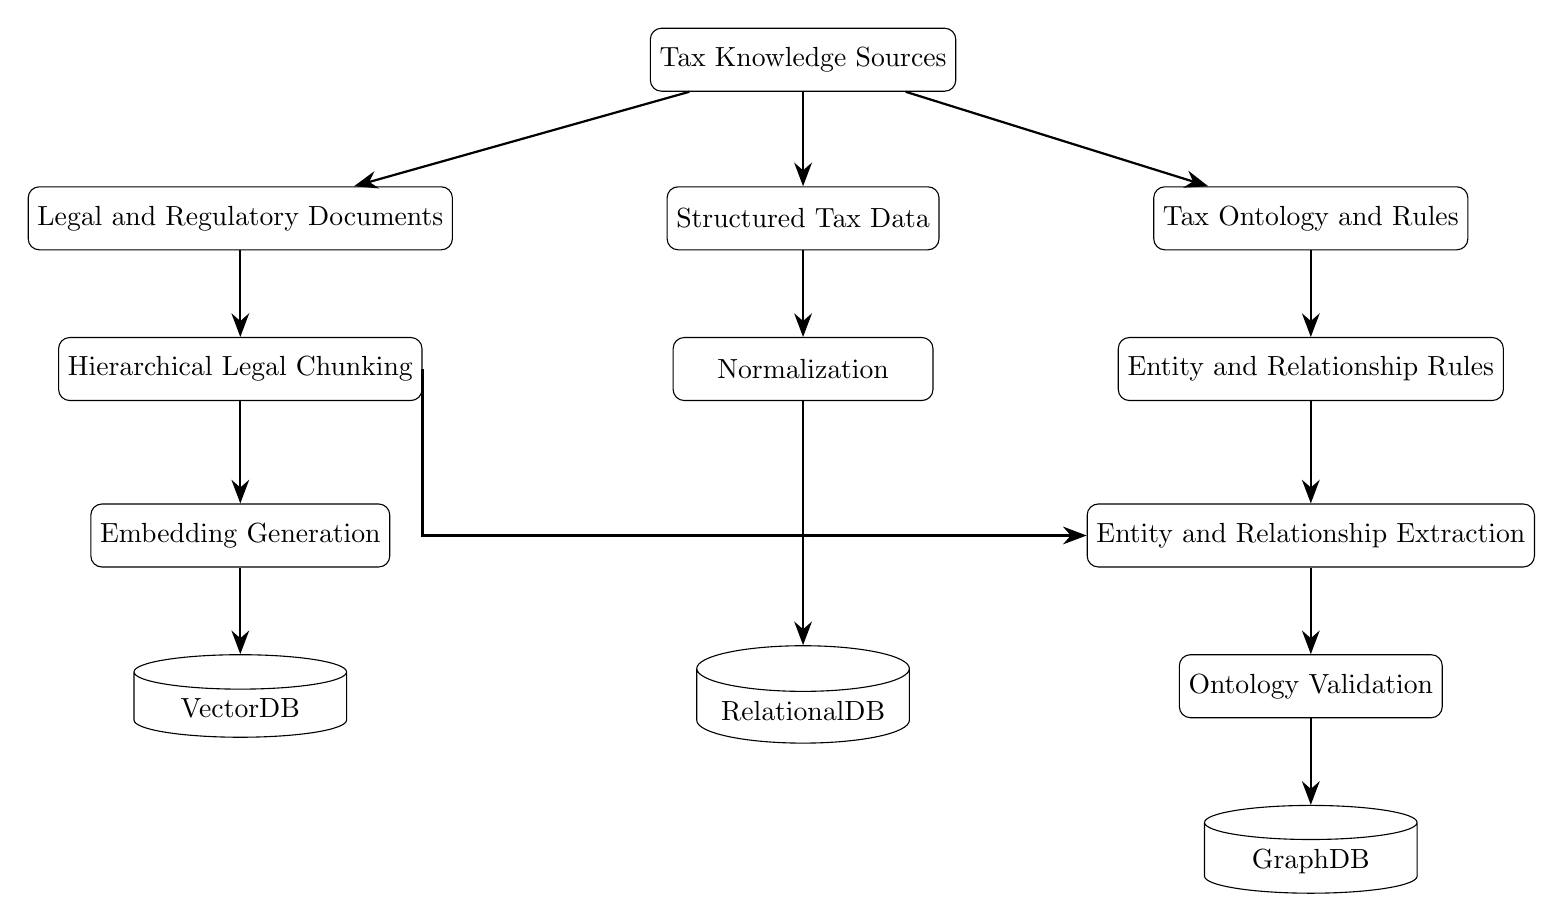
\begin{tikzpicture}[node distance=1.1cm and 2cm]
\node[process](src){Tax Knowledge Sources};
\node[process,below left=1.2cm and 2.5cm of src](docs){Legal and Regulatory Documents};
\node[process,below=1.2cm of src](struct){Structured Tax Data};
\node[process,below right=1.2cm and 2.5cm of src](onto){Tax Ontology and Rules};
\node[process,below=of docs](chunk){Hierarchical Legal Chunking};
\node[process,below=of struct](norm){Normalization};
\node[process,below=of onto](rules){Entity and Relationship Rules};
\node[process,below=1.3cm of chunk](embed){Embedding Generation};
\node[datastore,below=of embed](vdb){VectorDB};
\node[process,below=1.3cm of rules](extract){Entity and Relationship Extraction};
\node[process,below=of extract](validate){Ontology Validation};
\node[datastore,below=of validate](gdb){GraphDB};
\node[datastore,below=3.1cm of norm](rdb){RelationalDB};
\draw[flow](src)--(docs);\draw[flow](src)--(struct);\draw[flow](src)--(onto);
\draw[flow](docs)--(chunk);\draw[flow](struct)--(norm);\draw[flow](onto)--(rules);
\draw[flow](chunk)--(embed);\draw[flow](embed)--(vdb);
\draw[flow](chunk.east)|-(extract.west);\draw[flow](rules)--(extract);\draw[flow](extract)--(validate);\draw[flow](validate)--(gdb);
\draw[flow](norm)--(rdb);
\end{tikzpicture}
\end{center}

\section{Knowledge Domains and Vector Namespaces}
A single physical VectorDB may use namespaces, collections, or metadata partitions:
\begin{lstlisting}
tax-law/
+-- india/
+-- united-states/
+-- germany/
+-- united-kingdom/
+-- singapore/
+-- uae/
+-- other-jurisdictions/
+-- treaties/
+-- international-tax/
+-- reporting/
\end{lstlisting}
The GraphDB determines which namespaces are relevant to a cross-border fact pattern.

\section{Graph Ontology}
The initial ontology should remain deliberately small. Its purpose is retrieval orchestration, not an attempt to model all global tax law.

\subsection{Primary Entities}
\begin{center}
\begin{tabular}{p{3.5cm}p{9cm}}\toprule
Entity & Examples\\\midrule
Taxpayer & Individual, company, trust, partnership\\
Tax Residence & Resident, non-resident, jurisdiction-specific status\\
Jurisdiction & India, United States, Germany, Singapore\\
Asset & Equity, real estate, bond, bank account, retirement account\\
Income & Dividend, interest, capital gain, rental income, royalty\\
Tax Event & Sale, distribution, vesting, exercise, redemption\\
Tax Rule & Statute, regulation, administrative rule\\
Tax Treaty & Bilateral or multilateral agreement\\
Treaty Article & Dividend, capital gain, or relief article\\
Tax Credit & Foreign tax credit or related relief\\
Refund Mechanism & Withholding refund or recovery procedure\\
Reporting Requirement & Foreign asset or tax-return disclosure\\\bottomrule
\end{tabular}
\end{center}

\subsection{Core Relationships}
\begin{lstlisting}
Taxpayer --TAX_RESIDENT_OF--> Jurisdiction
Taxpayer --OWNS--> Asset
Asset --LOCATED_IN--> Jurisdiction
Asset --GENERATES--> Income
Income --TAXABLE_IN--> Jurisdiction
Income --SOURCE_TAXABLE_IN--> Jurisdiction
Tax --WITHHELD_BY--> Jurisdiction
Jurisdiction --HAS_TREATY_WITH--> Jurisdiction
Treaty --CONTAINS--> Treaty Article
Foreign Tax Paid --MAY_QUALIFY_FOR--> Foreign Tax Credit
Taxpayer --SUBJECT_TO--> Reporting Requirement
Tax Rule --APPLIES_TO--> Income
\end{lstlisting}

\section{Reference Graph: Indian Resident with US Equity}
\begin{center}
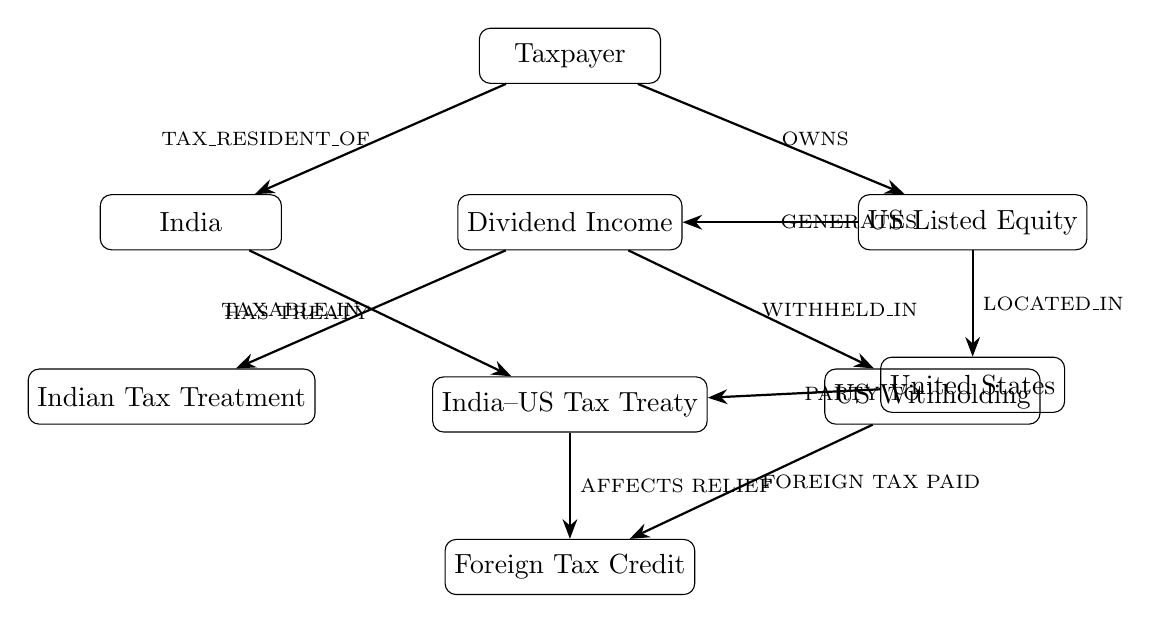
\begin{tikzpicture}[node distance=1.35cm and 2.2cm]
\node[entity](taxpayer){Taxpayer};
\node[entity,below left=1.4cm and 2.5cm of taxpayer](india){India};
\node[entity,below right=1.4cm and 2.5cm of taxpayer](equity){US Listed Equity};
\node[entity,below=of equity](us){United States};
\node[entity,below=1.4cm of taxpayer](dividend){Dividend Income};
\node[entity,below left=1.5cm and 1.8cm of dividend](indtax){Indian Tax Treatment};
\node[entity,below right=1.5cm and 1.8cm of dividend](ustax){US Withholding};
\node[entity,below=1.6cm of dividend](treaty){India--US Tax Treaty};
\node[entity,below=of treaty](credit){Foreign Tax Credit};
\draw[relation](taxpayer)--node[left,font=\scriptsize]{TAX\_RESIDENT\_OF}(india);
\draw[relation](taxpayer)--node[right,font=\scriptsize]{OWNS}(equity);
\draw[relation](equity)--node[right,font=\scriptsize]{LOCATED\_IN}(us);
\draw[relation](equity)--node[right,font=\scriptsize]{GENERATES}(dividend);
\draw[relation](dividend)--node[left,font=\scriptsize]{TAXABLE\_IN}(indtax);
\draw[relation](dividend)--node[right,font=\scriptsize]{WITHHELD\_IN}(ustax);
\draw[relation](india)--node[left,font=\scriptsize]{HAS TREATY}(treaty);
\draw[relation](us)--node[right,font=\scriptsize]{PARTY TO}(treaty);
\draw[relation](ustax)--node[right,font=\scriptsize]{FOREIGN TAX PAID}(credit);
\draw[relation](treaty)--node[right,font=\scriptsize]{AFFECTS RELIEF}(credit);
\end{tikzpicture}
\end{center}

The graph does not itself determine final tax liability. It identifies the legal neighborhoods that should participate in evidence retrieval.

\section{Chunking Strategy}
Fixed-size chunking alone is insufficient because legal provisions depend on hierarchy, provisos, exceptions, definitions, cross-references, and effective dates.

The recommended structure is hierarchical:
\begin{center}
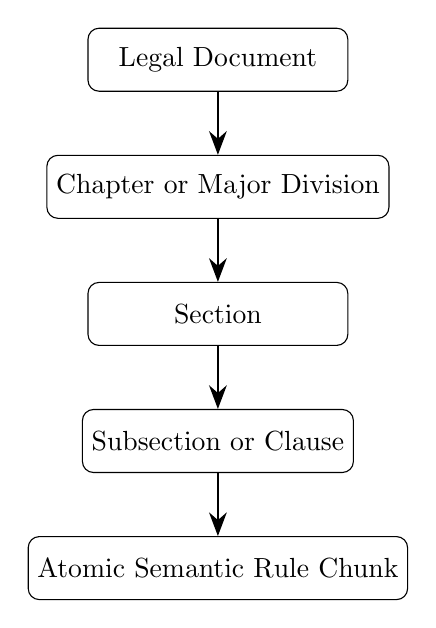
\begin{tikzpicture}[node distance=.8cm]
\node[process](d){Legal Document};
\node[process,below=of d](c){Chapter or Major Division};
\node[process,below=of c](s){Section};
\node[process,below=of s](ss){Subsection or Clause};
\node[process,below=of ss](a){Atomic Semantic Rule Chunk};
\draw[flow](d)--(c);\draw[flow](c)--(s);\draw[flow](s)--(ss);\draw[flow](ss)--(a);
\end{tikzpicture}
\end{center}

Example metadata:
\begin{lstlisting}
chunk_id: IN_CAP_GAIN_001
jurisdiction: India
tax_domain: Capital Gains
income_type: Capital Gain
asset_type: Listed Equity
taxpayer_type: Individual
legal_source: Income Tax Act
section: ...
effective_from: YYYY-MM-DD
effective_to: null
authority_level: Primary
entity_ids:
  - jurisdiction_india
  - income_capital_gain
  - asset_listed_equity
\end{lstlisting}

\section{Enrichment Strategy}
Each chunk should be enriched with:
\begin{itemize}
\item jurisdiction and tax authority;
\item legal hierarchy;
\item tax domain, income type, and asset type;
\item taxpayer category;
\item effective period;
\item authority level;
\item canonical entity identifiers;
\item source document and section provenance.
\end{itemize}

Asset normalization can map user language to legal categories:
\begin{center}
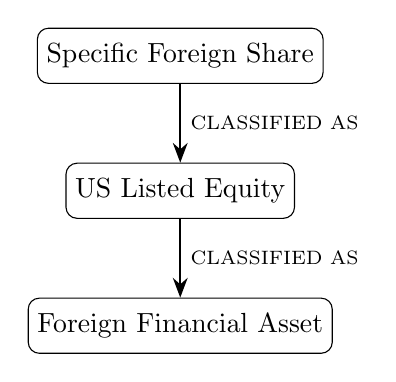
\begin{tikzpicture}[node distance=1cm]
\node[entity](specific){Specific Foreign Share};
\node[entity,below=of specific](listed){US Listed Equity};
\node[entity,below=of listed](foreign){Foreign Financial Asset};
\draw[relation](specific)--node[right,font=\scriptsize]{CLASSIFIED AS}(listed);
\draw[relation](listed)--node[right,font=\scriptsize]{CLASSIFIED AS}(foreign);
\end{tikzpicture}
\end{center}

\section{Local Plain RAG Workflow}
\begin{center}
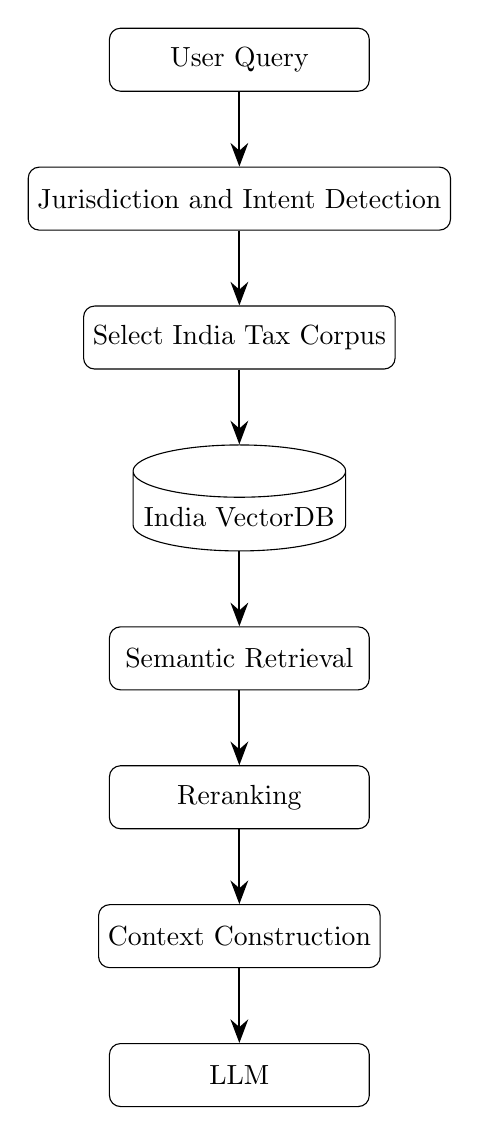
\begin{tikzpicture}[node distance=.95cm]
\node[process](q){User Query};
\node[process,below=of q](classify){Jurisdiction and Intent Detection};
\node[process,below=of classify](select){Select India Tax Corpus};
\node[datastore,below=of select](v){India VectorDB};
\node[process,below=of v](retrieve){Semantic Retrieval};
\node[process,below=of retrieve](rerank){Reranking};
\node[process,below=of rerank](ctx){Context Construction};
\node[process,below=of ctx](llm){LLM};
\draw[flow](q)--(classify);\draw[flow](classify)--(select);\draw[flow](select)--(v);
\draw[flow](v)--(retrieve);\draw[flow](retrieve)--(rerank);\draw[flow](rerank)--(ctx);\draw[flow](ctx)--(llm);
\end{tikzpicture}
\end{center}

\section{Cross-Border Graph-RAG Workflow}
\begin{center}
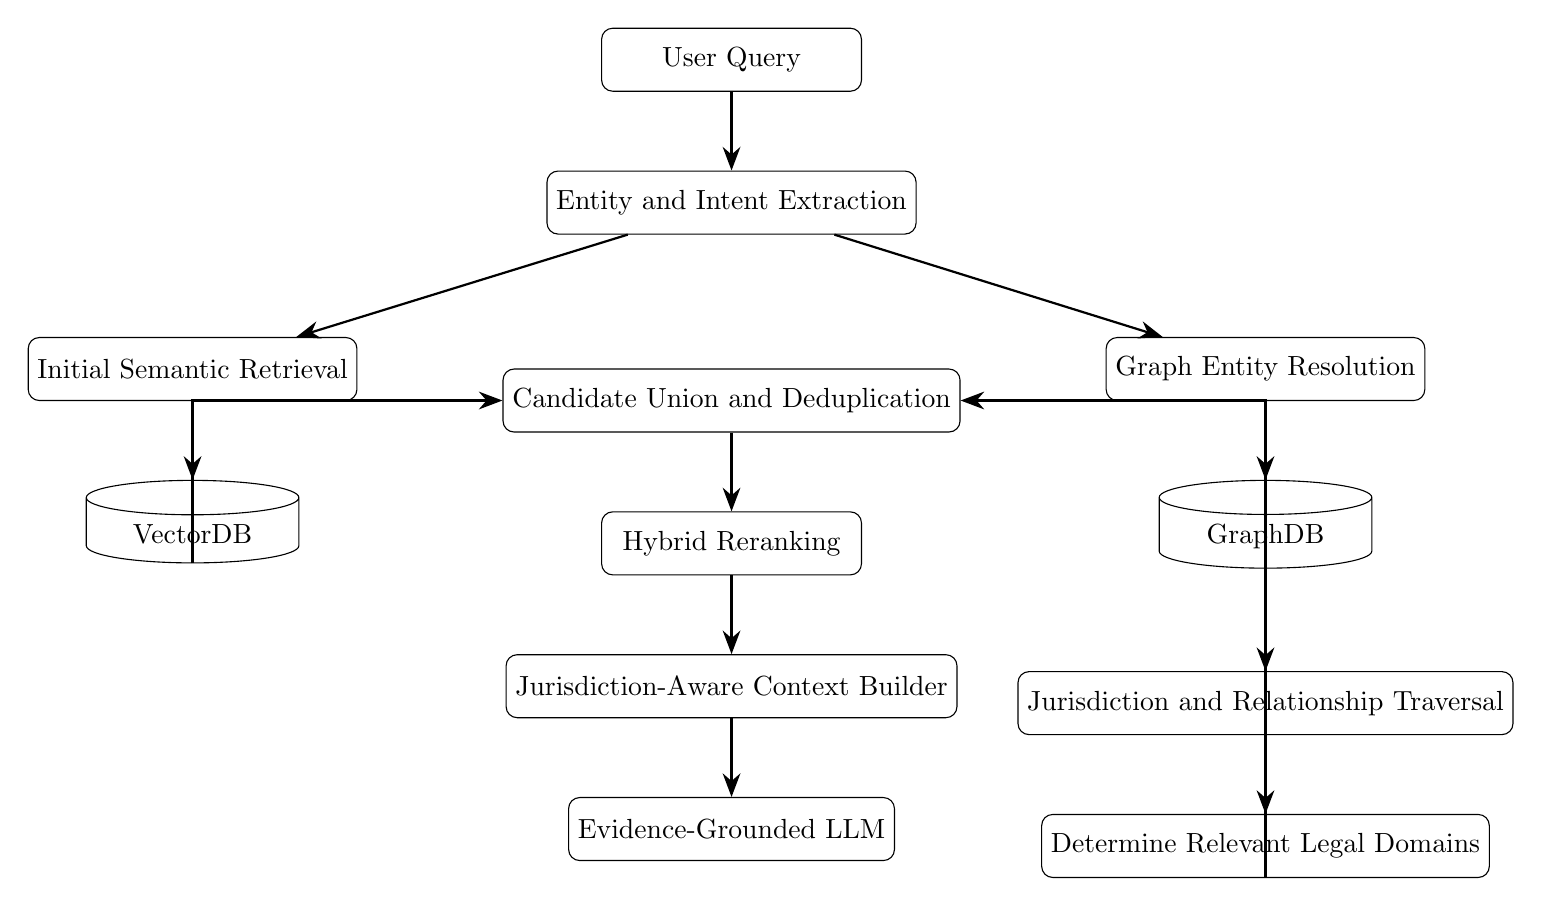
\begin{tikzpicture}[node distance=1cm and 2.8cm]
\node[process](q){User Query};
\node[process,below=of q](analysis){Entity and Intent Extraction};
\node[process,below left=1.3cm and 2.4cm of analysis](vs){Initial Semantic Retrieval};
\node[process,below right=1.3cm and 2.4cm of analysis](er){Graph Entity Resolution};
\node[datastore,below=of vs](vdb){VectorDB};
\node[datastore,below=of er](gdb){GraphDB};
\node[process,below=1.3cm of gdb](trav){Jurisdiction and Relationship Traversal};
\node[process,below=of trav](plan){Determine Relevant Legal Domains};
\node[process,below=1.7cm of analysis](fusion){Candidate Union and Deduplication};
\node[process,below=of fusion](rank){Hybrid Reranking};
\node[process,below=of rank](context){Jurisdiction-Aware Context Builder};
\node[process,below=of context](llm){Evidence-Grounded LLM};
\draw[flow](q)--(analysis);\draw[flow](analysis)--(vs);\draw[flow](analysis)--(er);
\draw[flow](vs)--(vdb);\draw[flow](er)--(gdb);\draw[flow](gdb)--(trav);\draw[flow](trav)--(plan);
\draw[flow](vdb.south)|-(fusion.west);\draw[flow](plan.south)|-(fusion.east);
\draw[flow](fusion)--(rank);\draw[flow](rank)--(context);\draw[flow](context)--(llm);
\end{tikzpicture}
\end{center}

\section{Query Routing Logic}
\begin{center}
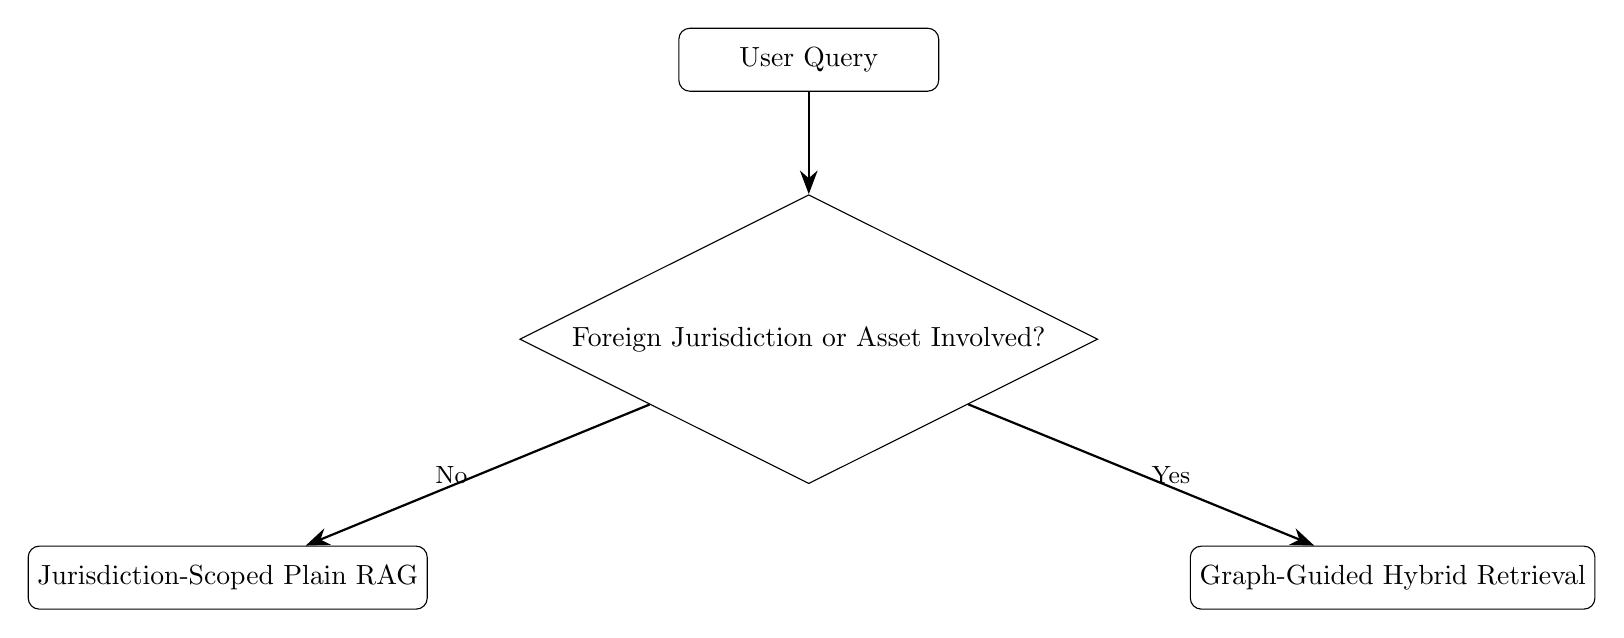
\begin{tikzpicture}[node distance=1.3cm and 3cm]
\node[process](q){User Query};
\node[decision,below=of q](f){Foreign Jurisdiction or Asset Involved?};
\node[process,below left=1.7cm and 3cm of f](local){Jurisdiction-Scoped Plain RAG};
\node[process,below right=1.7cm and 3cm of f](cross){Graph-Guided Hybrid Retrieval};
\draw[flow](q)--(f);\draw[flow](f)--node[left,font=\small]{No}(local);\draw[flow](f)--node[right,font=\small]{Yes}(cross);
\end{tikzpicture}
\end{center}
Suggested classes:
\begin{lstlisting}
LOCAL
CROSS_BORDER
MULTI_JURISDICTION
TREATY_RELATED
FOREIGN_TAX_CREDIT
FOREIGN_ASSET_REPORTING
FOREIGN_REFUND
\end{lstlisting}

\section{Graph-Guided Jurisdiction Expansion}
For an Indian resident holding a foreign asset, traversal can identify:
\begin{enumerate}
\item residence jurisdiction;
\item asset or source jurisdiction;
\item relevant income type;
\item connected treaty;
\item foreign withholding or source taxation;
\item domestic treatment;
\item foreign tax credit or refund mechanisms;
\item reporting obligations.
\end{enumerate}

The retrieval plan may therefore become:
\begin{lstlisting}
Search India Tax Corpus
+
Search Foreign Jurisdiction Tax Corpus
+
Search Bilateral Treaty Corpus
+
Search Foreign Tax Credit Corpus
+
Search Reporting / Documentation Corpus
\end{lstlisting}

This is the central Graph-RAG advantage: the graph makes the required knowledge expansion explicit instead of hoping every necessary jurisdictional document ranks highly in a global semantic search.

\section{Candidate Generation and Fusion}
Let:
\[
C=C_{\text{vector}}\cup C_{\text{graph}}\cup C_{\text{structured}}.
\]
Here:
\begin{itemize}
\item $C_{\text{vector}}$ contains semantic candidates;
\item $C_{\text{graph}}$ contains evidence linked to relevant entities and graph paths;
\item $C_{\text{structured}}$ contains exact rules, dates, thresholds, or other deterministic records.
\end{itemize}

Every candidate should preserve provenance:
\begin{lstlisting}
chunk_id
source_corpus
jurisdiction
entity_ids
graph_path
vector_score
effective_from
effective_to
authority_level
source_document_id
section_reference
\end{lstlisting}

\section{Hybrid Ranking}
A conceptual score is:
\[
Score(c)=\alpha S_v(c)+\beta S_g(c)+\gamma S_j(c)+\delta S_t(c)+\epsilon S_a(c)
\]
where:
\begin{itemize}
\item $S_v$ is semantic relevance;
\item $S_g$ is graph or path relevance;
\item $S_j$ is jurisdiction relevance;
\item $S_t$ is temporal validity;
\item $S_a$ is source authority.
\end{itemize}
In practice, candidate generation followed by a dedicated reranker may be easier to maintain than a heavily hand-tuned formula.

\section{Temporal Validity and Authority}
Tax law is time-dependent. Candidate retrieval must identify the relevant tax period and filter or deprioritize rules outside that period.
\begin{center}
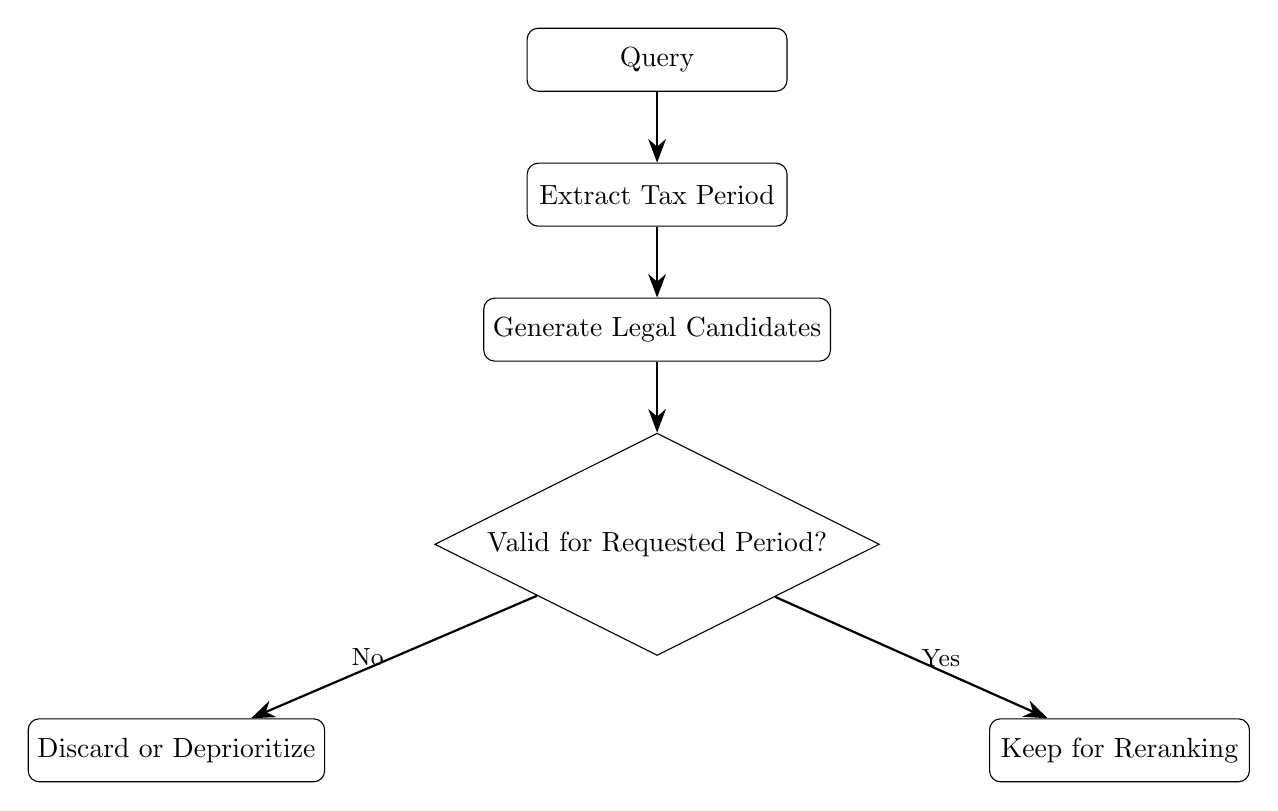
\begin{tikzpicture}[node distance=.9cm]
\node[process](q){Query};
\node[process,below=of q](date){Extract Tax Period};
\node[process,below=of date](cand){Generate Legal Candidates};
\node[decision,below=of cand](valid){Valid for Requested Period?};
\node[process,below left=1.5cm and 2.8cm of valid](drop){Discard or Deprioritize};
\node[process,below right=1.5cm and 2.8cm of valid](keep){Keep for Reranking};
\draw[flow](q)--(date);\draw[flow](date)--(cand);\draw[flow](cand)--(valid);
\draw[flow](valid)--node[left,font=\small]{No}(drop);\draw[flow](valid)--node[right,font=\small]{Yes}(keep);
\end{tikzpicture}
\end{center}
A conceptual authority hierarchy is:
\[
\text{Primary Statute/Treaty}
>
\text{Regulation}
>
\text{Tax Authority Guidance}
>
\text{Official Procedure}
>
\text{Secondary Commentary}.
\]

\section{Structured Context Construction}
The final prompt context should be organized by legal role rather than as one mixed list of chunks:
\begin{lstlisting}
QUESTION

FACT PATTERN
Taxpayer Residence: ...
Asset Jurisdiction: ...
Asset Type: ...
Income: ...
Foreign Tax Event: ...

RELEVANT GRAPH PATH

SOURCE-JURISDICTION EVIDENCE

RESIDENCE-JURISDICTION EVIDENCE

TREATY EVIDENCE

FOREIGN TAX CREDIT / RELIEF EVIDENCE

REFUND EVIDENCE

REPORTING REQUIREMENTS

MISSING FACTS AND CONDITIONS
\end{lstlisting}

\section{Cross-Store Linkage}
All stores should use stable canonical identifiers:
\begin{center}
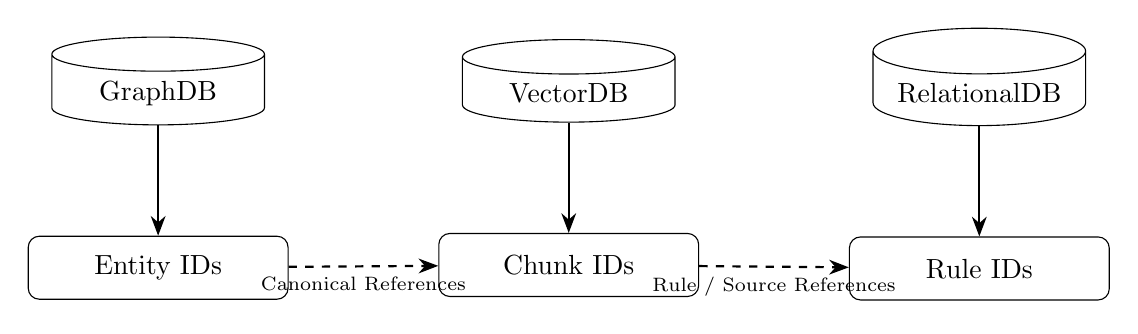
\begin{tikzpicture}[node distance=1.5cm and 2.5cm]
\node[datastore](g){GraphDB};
\node[datastore,right=of g](v){VectorDB};
\node[datastore,right=of v](r){RelationalDB};
\node[process,below=1.4cm of g](eid){Entity IDs};
\node[process,below=1.4cm of v](cid){Chunk IDs};
\node[process,below=1.4cm of r](rid){Rule IDs};
\draw[relation](g)--(eid);\draw[relation](v)--(cid);\draw[relation](r)--(rid);
\draw[relation,dashed](eid)--node[below,font=\scriptsize]{Canonical References}(cid);
\draw[relation,dashed](cid)--node[below,font=\scriptsize]{Rule / Source References}(rid);
\end{tikzpicture}
\end{center}

This supports both:
\[
\text{Graph Entity}\rightarrow\text{Supporting Chunks}
\]
and:
\[
\text{Chunk}\rightarrow\text{Entities}\rightarrow\text{Graph Neighborhood}.
\]

\section{Plain RAG versus Graph-RAG}
\begin{longtable}{p{3.2cm}p{5.5cm}p{5.5cm}}\toprule
Capability & Plain RAG & Graph-RAG\\\midrule
\endhead
Primary signal & Semantic similarity & Semantic similarity plus relationship structure\\
Jurisdiction selection & Query-driven & Graph-guided expansion\\
Cross-border links & Implicit in text & Explicitly modeled\\
Treaty discovery & Similarity-dependent & Traversable jurisdiction relationships\\
Asset classification & Metadata or inference & Graph taxonomy\\
Multi-hop analysis & Depends on retrieving all passages & Paths identify connected domains\\
Candidate expansion & Top-K similarity & Vector plus graph-derived candidates\\
Context & Ranked chunks & Jurisdiction and path-aware evidence\\
Explainability & Passage provenance & Passage plus relationship-path provenance\\
\bottomrule
\end{longtable}

\section{Evaluation}
Evaluation should compare local and cross-border query classes:
\begin{itemize}
\item local factual retrieval;
\item cross-border taxation;
\item treaty-related retrieval;
\item foreign tax credit;
\item foreign asset reporting;
\item refund analysis;
\item multi-hop dependency;
\item historical tax-period queries.
\end{itemize}
Metrics should include Context Precision, Context Recall, Entity Resolution Accuracy, Relationship Precision and Recall, Graph Path Accuracy, Jurisdiction Coverage, Temporal Validity Accuracy, Source Authority Compliance, Answer Faithfulness, Answer Correctness, Latency, and Token Cost.

\section{Governance and Provenance}
Every material graph fact should ideally be traceable:
\begin{center}
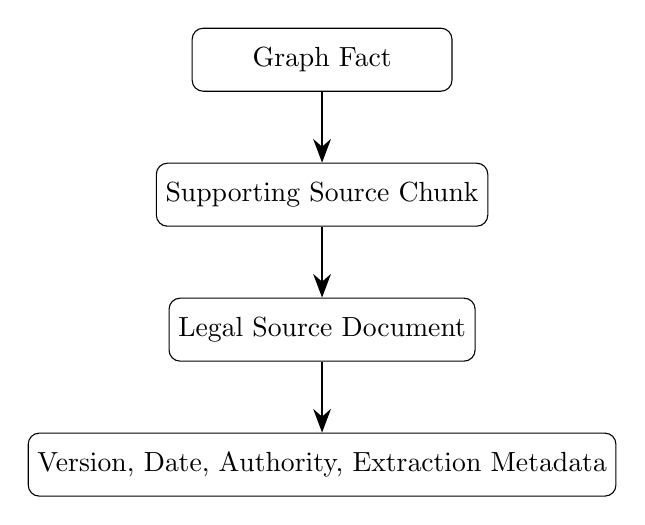
\begin{tikzpicture}[node distance=.9cm]
\node[process](fact){Graph Fact};
\node[process,below=of fact](chunk){Supporting Source Chunk};
\node[process,below=of chunk](doc){Legal Source Document};
\node[process,below=of doc](meta){Version, Date, Authority, Extraction Metadata};
\draw[flow](fact)--(chunk);\draw[flow](chunk)--(doc);\draw[flow](doc)--(meta);
\end{tikzpicture}
\end{center}
Recommended provenance:
\begin{lstlisting}
source_document_id
source_chunk_id
jurisdiction
legal_reference
effective_from / effective_to
authority_level
ontology_version
rulebook_version
extractor_version
confidence
ingestion_timestamp
\end{lstlisting}

\section{Phased Implementation Plan}
\subsection{Phase 1: India-Only Plain RAG}
Implement source ingestion, hierarchical chunking, metadata extraction, embeddings, VectorDB retrieval, reranking, evidence-grounded answers, and baseline evaluation.

\subsection{Phase 2: Add One Foreign Jurisdiction}
Add a controlled cross-border domain, for example:
\begin{lstlisting}
India + United States + India--US Treaty Corpus
\end{lstlisting}

\subsection{Phase 3: Add the Graph}
Start with:
\begin{lstlisting}
Taxpayer, Jurisdiction, Asset, Income,
Tax Event, Tax Rule, Treaty,
Tax Credit, Reporting Requirement
\end{lstlisting}

\subsection{Phase 4: Add Cross-Store Linkage}
Connect graph nodes, vector metadata, structured records, and source documents through canonical IDs.

\subsection{Phase 5: Add Query Routing}
\begin{lstlisting}
LOCAL -> scoped Vector RAG
CROSS_BORDER -> Graph-guided hybrid retrieval
TREATY_RELATED -> graph traversal + treaty retrieval
FOREIGN_TAX_CREDIT -> domestic + foreign + treaty retrieval
FOREIGN_ASSET_REPORTING -> asset graph + reporting retrieval
\end{lstlisting}

\subsection{Phase 6: Parallel Hybrid Retrieval}
Implement semantic retrieval, entity resolution, graph traversal, jurisdiction expansion, structured retrieval, candidate union, and deduplication.

\subsection{Phase 7: Ranking and Context}
Add temporal filtering, authority weighting, graph relevance, reranking, jurisdiction-aware context construction, provenance, and missing-fact detection.

\subsection{Phase 8: Regression Evaluation}
Version and evaluate changes to ontology, extraction rules, embedding models, retrieval logic, traversal logic, rerankers, and context construction.

\section{Reference Repository Structure}
\begin{lstlisting}
cross-border-tax-rag/
+-- schemas/
|   +-- tax_ontology.yaml
|   +-- graph_schema.yaml
+-- rules/
|   +-- entity_rules.yaml
|   +-- relationship_rules.yaml
+-- sources/
|   +-- india/
|   +-- united_states/
|   +-- treaties/
+-- ingestion/
|   +-- legal_parser.py
|   +-- chunker.py
|   +-- metadata_extractor.py
|   +-- entity_extractor.py
|   +-- relationship_extractor.py
|   +-- validator.py
+-- storage/
|   +-- vector_store.py
|   +-- graph_store.py
|   +-- relational_store.py
+-- retrieval/
|   +-- query_classifier.py
|   +-- entity_resolver.py
|   +-- vector_retriever.py
|   +-- graph_retriever.py
|   +-- structured_retriever.py
|   +-- candidate_fusion.py
|   +-- temporal_filter.py
|   +-- authority_filter.py
|   +-- reranker.py
+-- context/
|   +-- context_builder.py
|   +-- provenance.py
+-- evaluation/
|   +-- datasets/
|   +-- retrieval_eval.py
|   +-- graph_eval.py
|   +-- regression_tests/
\end{lstlisting}

\section{Final Reference Architecture}
\begin{center}
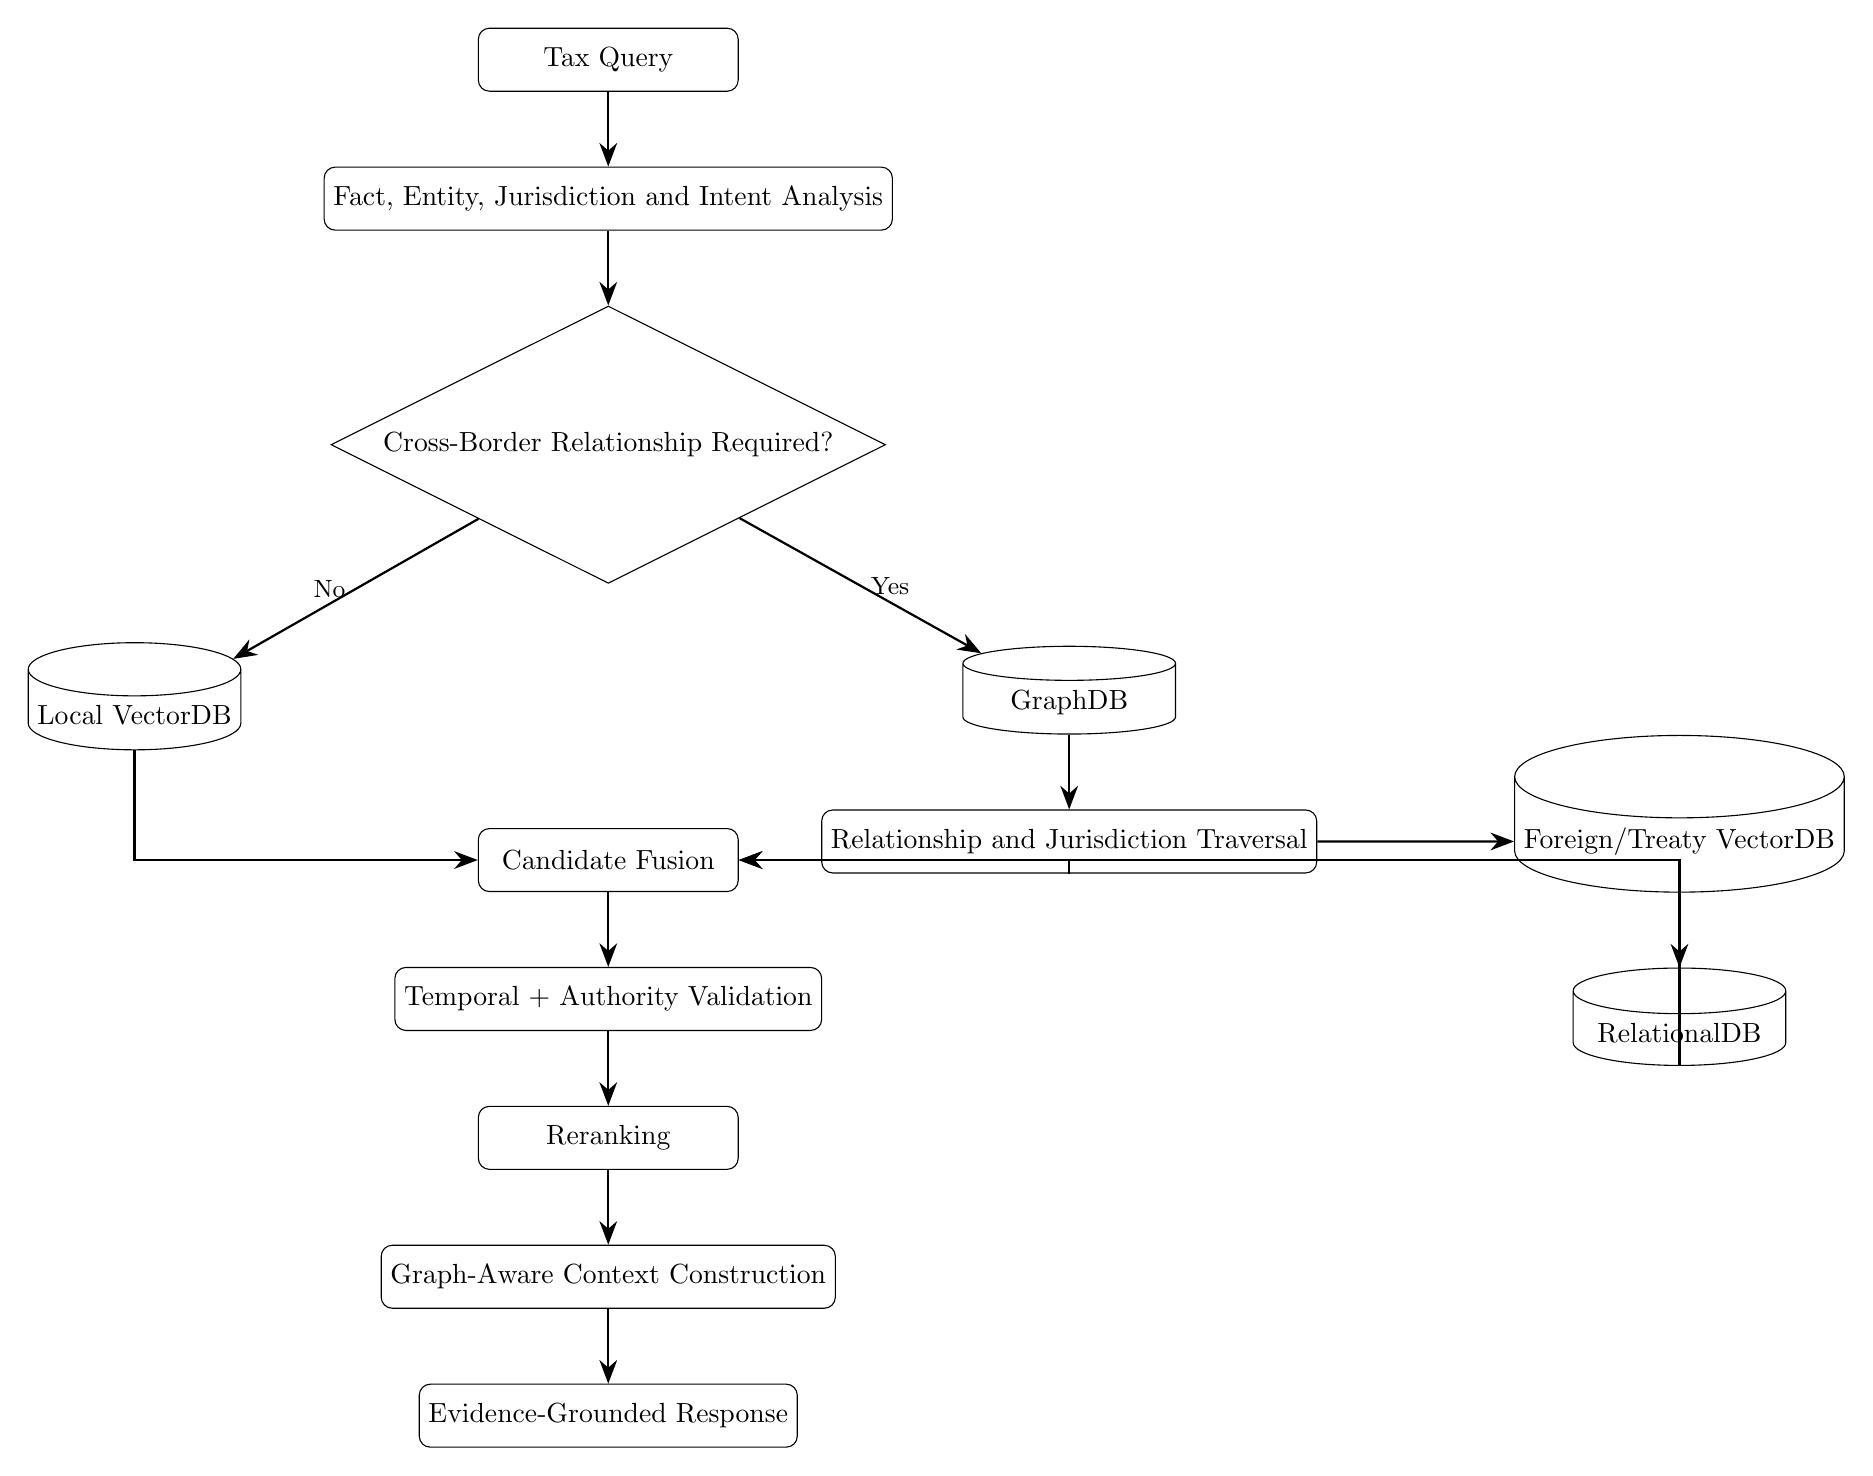
\begin{tikzpicture}[node distance=.95cm and 2.1cm]
\node[process](q){Tax Query};
\node[process,below=of q](analysis){Fact, Entity, Jurisdiction and Intent Analysis};
\node[decision,below=of analysis](d){Cross-Border Relationship Required?};
\node[datastore,below left=1.7cm and 3.4cm of d](local){Local VectorDB};
\node[datastore,below right=1.7cm and 3.4cm of d](gdb){GraphDB};
\node[process,below=of gdb](trav){Relationship and Jurisdiction Traversal};
\node[datastore,right=2.5cm of trav](foreign){Foreign/Treaty VectorDB};
\node[datastore,below=of foreign](rdb){RelationalDB};
\node[process,below=3.1cm of d](fusion){Candidate Fusion};
\node[process,below=of fusion](valid){Temporal + Authority Validation};
\node[process,below=of valid](rank){Reranking};
\node[process,below=of rank](ctx){Graph-Aware Context Construction};
\node[process,below=of ctx](llm){Evidence-Grounded Response};
\draw[flow](q)--(analysis);\draw[flow](analysis)--(d);
\draw[flow](d)--node[left,font=\small]{No}(local);
\draw[flow](d)--node[right,font=\small]{Yes}(gdb);
\draw[flow](gdb)--(trav);\draw[flow](trav)--(foreign);\draw[flow](foreign)--(rdb);
\draw[flow](local.south)|-(fusion.west);
\draw[flow](trav.south)|-(fusion.east);
\draw[flow](rdb.south)|-(fusion.east);
\draw[flow](fusion)--(valid);\draw[flow](valid)--(rank);\draw[flow](rank)--(ctx);\draw[flow](ctx)--(llm);
\end{tikzpicture}
\end{center}

\section{Summary}
A jurisdiction-local tax question can often use scoped semantic retrieval. A cross-border question requires the retrieval system to identify and connect residence jurisdiction, asset location, source-country treatment, residence-country treatment, treaty relationships, foreign tax paid, possible relief, refund paths, reporting obligations, effective dates, and source authority.

The GraphDB supplies the structural model used to determine the retrieval neighborhood. The VectorDB retrieves source-backed legal evidence from that neighborhood. The RelationalDB provides exact structured values and temporal parameters. The retrieval orchestration layer fuses these signals, validates legal applicability, reranks evidence, and builds a structured context for the language model.

\end{document}
